\documentclass[a4paper,12pt,titlepage]{article}
\pagestyle{plain} 

\usepackage[left=3cm,right=1cm,
    top=2cm,bottom=2cm,bindingoffset=0cm]{geometry}

\linespread{1.3}



\usepackage[T2A]{fontenc}
\usepackage[utf8]{inputenc}
\usepackage[russian]{babel}
\usepackage{amsmath, amssymb, amsfonts}
\usepackage{graphicx}
\usepackage{epsfig}
\usepackage{wrapfig}
\usepackage{floatflt}
\usepackage{array}
\usepackage{hhline}
\usepackage{longtable}
\usepackage{multirow}
\usepackage{mathrsfs}
\usepackage[unicode, pdftex]{hyperref}
\usepackage{amsthm}

\usepackage{pscyr}


\usepackage{setspace}

\theoremstyle{definition}
\newtheorem{definition}{Определение}

\theoremstyle{theorem}
\newtheorem{theorem}{Теорема}


\theoremstyle{definition}
\newtheorem{Proposition}{Предложение} 


\begin{document}
\thispagestyle{empty}
\begin{center}
    \large
Государственное бюджетное образовательное учреждение
высшего образования Московской области

«Университет «Дубна»\\[15pt]

Инженерно-физический институт

Кафедра фундументальных проблем физики микромира\\[15pt]

Курсовая работа по 

Теме:\\[15pt]

«Колебательные процессы»\\[105pt]
\end{center}

\begin{flushright}
Выполнил:

студент группы 3161

Баки Даниил Феликсович

Преподаватель:

кандидат физ.-мат. наук, доцент кафедры ядерной физики 

Рачков Владимир Александрович\\[250pt]

\end{flushright}

\begin{center}
    Дубна, 2022
\end{center}
\newpage
\begin{abstract}
    В работе исследуется механическая система состоящая из шарика закрепленного на двух 
    пружинах на поверхности стола. Для исследования данной системы были получены 
    уравнения движения для шарика и проведено математическое моделированное данной системы 
    с применением метода Рунге-Кутты четвертого порядка на языке программирования С++.
\end{abstract}
\tableofcontents
\newpage
\section{Введение}
Мы будем изучать колебательные процессы на следующем примере шарика 
 лежащего на горизонтальном столе, прикрепленом к двум пружинам с
жесткостями $k_x$ и $k_y$ и одинаковыми длинами $l$ в нерастянутом состоянии. 
Пружины взаимно
перпендикулярны в положении равновесия. В момент времени $t_0 = 0$ шарик оттягивают из
положения равновесия в точку с координатами $(x_0,\; y_0)$ 
относительно положения равновесия,
после чего отпускают. Моделью данной системы служит материальная точка, движущаяся 
на плоскости $(x,\; y) \in \mathbb{R}^2$ \\
\begin{figure}[h!!!]
    \noindent\centering{
        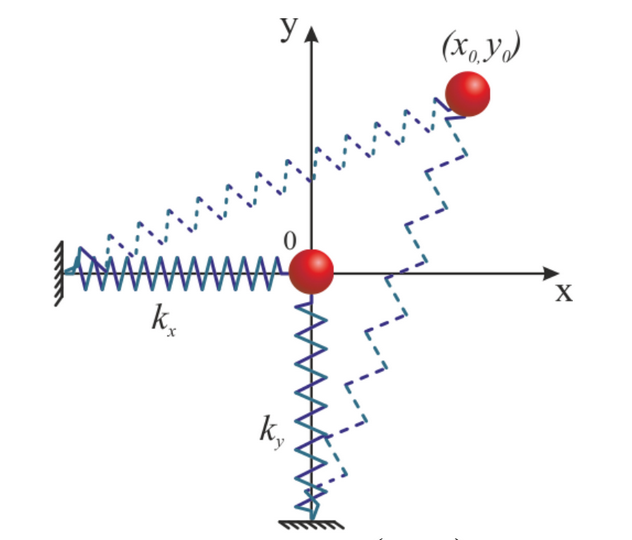
\includegraphics[width=0.49\linewidth]{usl.PNG}
    }
    \caption{Схема условия}
    \label{usl}
\end{figure}
\newpage
\section{Уравнения движения}\label{}
Лагранджиан нашей системы имеет вид:
\begin{equation}
    L = m\frac{\dot{x}^2 + \dot{y}^2}{2} - k_x\frac{x^2 + y^2}{2}
    - k_y\frac{x^2 + y^2}{2} - \frac{b}{2}\frac{d}{dt}\left(x^2 + y^2\right). 
\end{equation}
Чтобы уменьшить количество уравнений можно сделать замену $z = x + iy, \; z^* = x - iy$ 
и переписать:
\begin{equation}
    L = m\frac{\dot{z}\dot{z}^*}{2} - \left(k_x + k_y\right)\frac{zz^*}{2} 
    - \frac{b}{2}\frac{d}{dt}\left(zz^*\right).
\end{equation}
Из него получаем следующие уравнения движения:
\begin{equation}
    m\ddot{z} =  - \left(k_x + k_y\right)z - b\dot{z},
\end{equation}
где $b$ коэфициент силы трения.
Введем для удобства обозначения $A = (k_x + k_y)/m$ и 
$B = b / m$. Так же нам понадобиться разбить уравнения второго порядка 
на уравнения первого порядка. Для этого обозначим $v_z = \dot{z}$.
В итоге система имеет вид:
\begin{eqnarray}
    \dot{v_z} &=& -Az - Bv_z,\\
    \dot{z} &=& v_z.
\end{eqnarray}
Получим точное решение данной системы уранвений. Для этого будет удобно
фиксировать начальные условия $z(t = 0) = z_0$, $v_z(0) = v_0$ и использовать
матричную запись:
\begin{spacing}{1}
    \begin{equation}\label{matr}
        \dot{Z} = 
        \begin{pmatrix}
            \dot{v_z}\\
            \dot{z}
        \end{pmatrix}
        = 
        \begin{pmatrix}
            -B & -A \\
            1 & 0
        \end{pmatrix}
        \begin{pmatrix}
            v_z\\
            z
        \end{pmatrix}
        = MZ.
    \end{equation}
\end{spacing}
Собственные числа оператора $M$ будут:
\begin{equation}
    \lambda_{\pm} = \frac{-B \pm \sqrt{B^2 - 4A}}{2}.
\end{equation}
Собственный безис будет:
\begin{spacing}{1}
    \begin{equation}
        \xi_\pm = 
        \begin{pmatrix}
            \lambda_{\pm}\\
            1
        \end{pmatrix}
    \end{equation}
\end{spacing}
Тогда решение даеться следующей формулой (См. Гл.3 \S 17\cite{Arn}):
\begin{equation}
    Z(t) = e^{Mt}Z_0 = 
    \sum_{\pm} C_\pm e^{\lambda_{\pm}t}\xi_\pm,
\end{equation}
$C_{\pm}$ определяются из начальных условий.\\
Так как из определения констант следует $A, B > 0$, то из формулы выше следует, 
что собственные числа будут иметь отрицательную вещественную часть $\text{Re} (\lambda_{\pm}) < 0$. Так же они будут иметь 
ненулевую мнимую часть при выполнении условия
\begin{equation}\label{uslov}
    B^2 < 4A.
\end{equation}
Из классификации особых точкек ОДУ следует что при выполнении(или невыполнении) этого условия 
фазовые кривые будут иметь один из двух типов, представленных на Рис. \ref*{im}.
\begin{figure}[h!!!]

    \begin{minipage}[h]{0.40\linewidth}
    \center{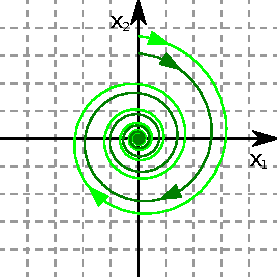
\includegraphics[width=1\linewidth]{logs.pdf} \\ Логарифмические спирали}
    \end{minipage}
    \hfill
    \begin{minipage}[h]{0.40\linewidth}
    \center{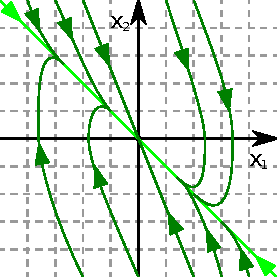
\includegraphics[width=1\linewidth]{pars.pdf} \\ Параболы}
    \end{minipage}
    \caption{Возможные фазовые партреты вблизи нуля\cite{log,par}}
    \label{im}
\end{figure}
Если же сила трения отсутствует, то $B = 0$, собственные числа чисто мнимые $\text{Re} (\lambda_{\pm}) = 0$,
что соответствует окружностям или гармоническим колебаниям, 
как на Рис. \ref*{cir}.

\begin{figure}[h!!!]

    \noindent\centering{
        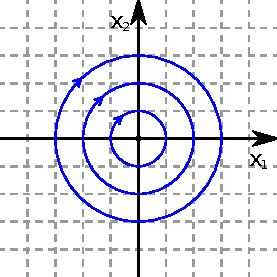
\includegraphics[width=0.40\linewidth]{re0.pdf}
    }
    \caption{Окружности на фазовом портрете при нулевой вещественной части собственных чисел \cite{cir}}
    \label{cir}
\end{figure}
Общая классификация представленна на Рис.\ref*{all}. В наших обозначениях 
$p = \text{Tr}\; M = -B, \; p = \det M = A, \; \Delta = B^2 - 4A$, 
где матрица $M$ береться из уравнения (\ref*{matr})
\begin{figure}[h!!!]

    \noindent\centering{
        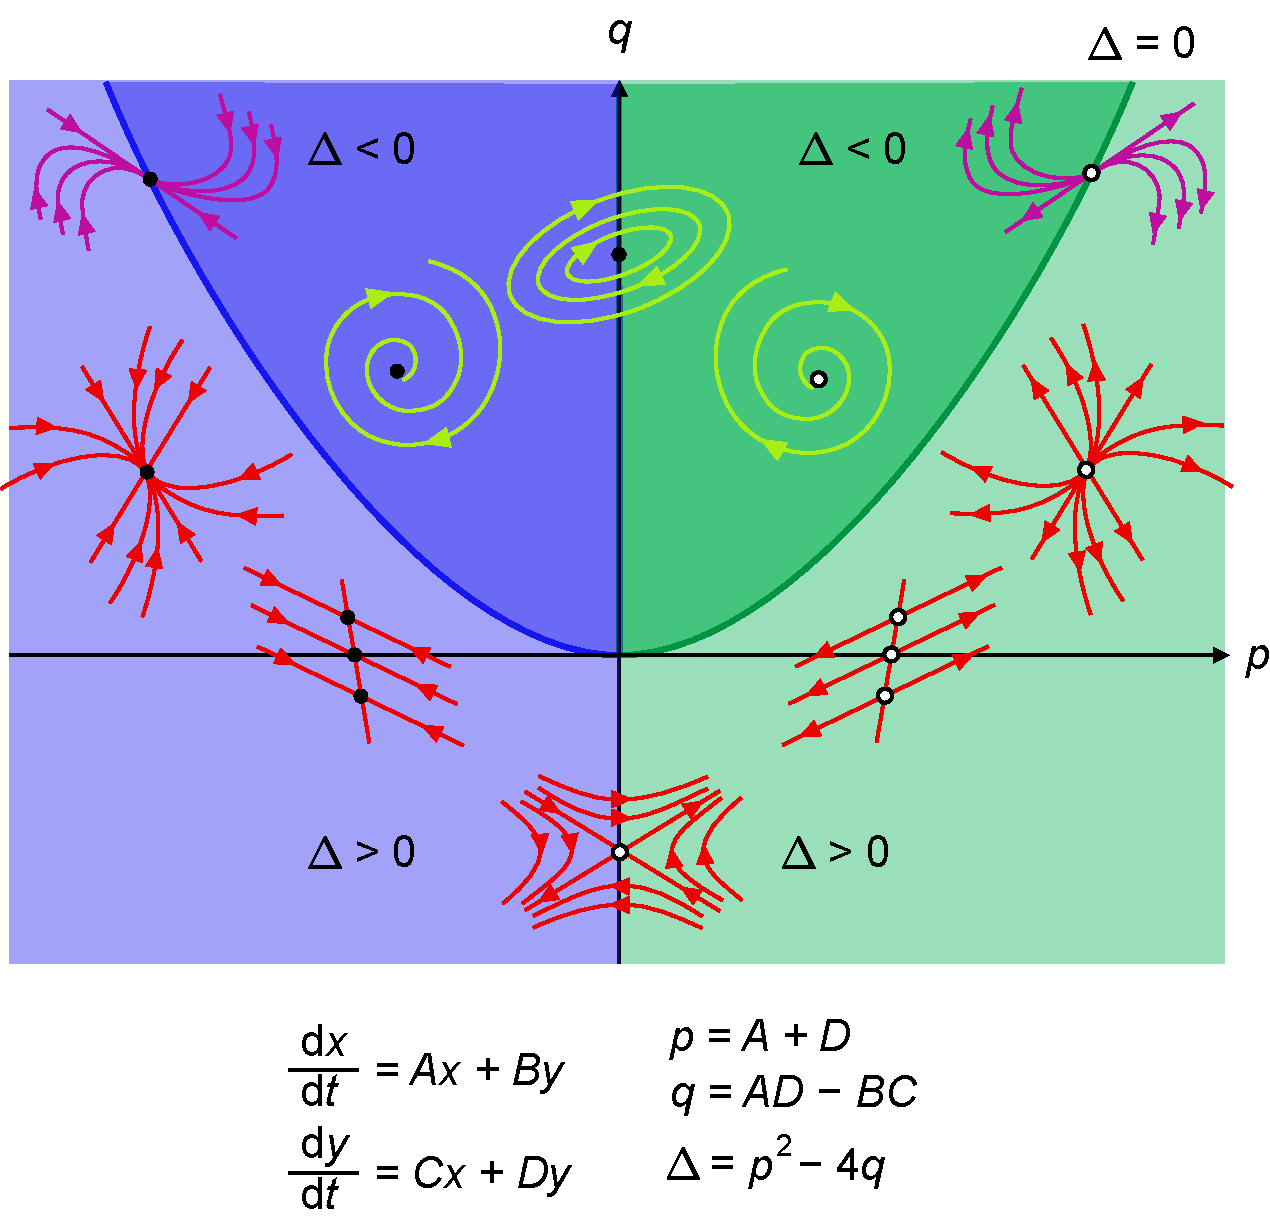
\includegraphics[width=0.6\linewidth]{all.pdf}
    }
    \caption{Все типы особых точек в завивисимости от Tr, $\det$ и $\Delta$ \cite{all}}
    \label{all}
\end{figure}


\newpage
\section{Метод Рунге-Кутты}
Пусть дана система из $n$ обыкновенных 
дифференциальных уравнений первого порядка:
\begin{eqnarray}
    \dot{X}  = F(t, X),
\end{eqnarray}
$X \in \mathbb{R}^n, t, h \in \mathbb{R}$, шаг сетки $h$  и начальное условие $X_0 = X(t = 0)$.
Для вычисления приблеженного решения в последующих точках требуется посчитать коэфициенты 
$k_i$(их получиться $4n$ штук -- на каждое уравнение системы по четыре $k_i$):
\begin{eqnarray}
    k_1 = F(&t_n,& X_n), \\
    k_2 = F(&t_n + h/2,& X_n + k_1h/2), \\
    k_3 = F(&t_n + h/2,& X_n + k_2h/2), \\
    k_4 = F(&t_n + h,& X_n + k_3h).
\end{eqnarray}
Тут индекс $n$ обозначет узел сетки.
Зная коэфициенты мы можем вычислить 
приближенное решение в следующей точке по следующей формуле:
\begin{equation}
    X_{n+1} = X_n + \frac{h}{6}(k_1 + 2k_2 + 2k_3 + k_4).
\end{equation}
Следует обратить внимание на двойки перед $k_2$ и $k_3$.
Суммарная ошибка на всем отрезке интегрирования будет порядка $O(h^4)$, 
поэтому метод и имеет четвертый 
порядок.
\newpage
\section{Результаты}
\subsection{Траектории}
\begin{figure}[h!!!]

    \noindent\centering{
        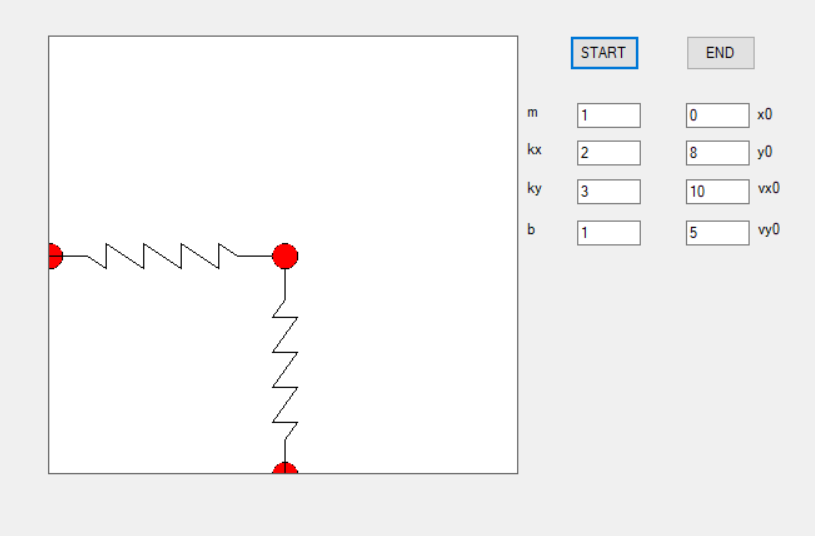
\includegraphics[width=0.9\linewidth]{Prog.PNG}
    }
    \caption{Окно с анимацией шарика с пружиной. Так же поля для ввода параметров}
    \label{prog}
\end{figure}
Далее будем приводить траектории шарика. 
Рассмотрим случай, когда трение отсутствует, тогда
траектория будет иметь вид эллипса как на Рис. \ref*{b0}.
\begin{figure}[h!!!]
    \noindent\centering{
        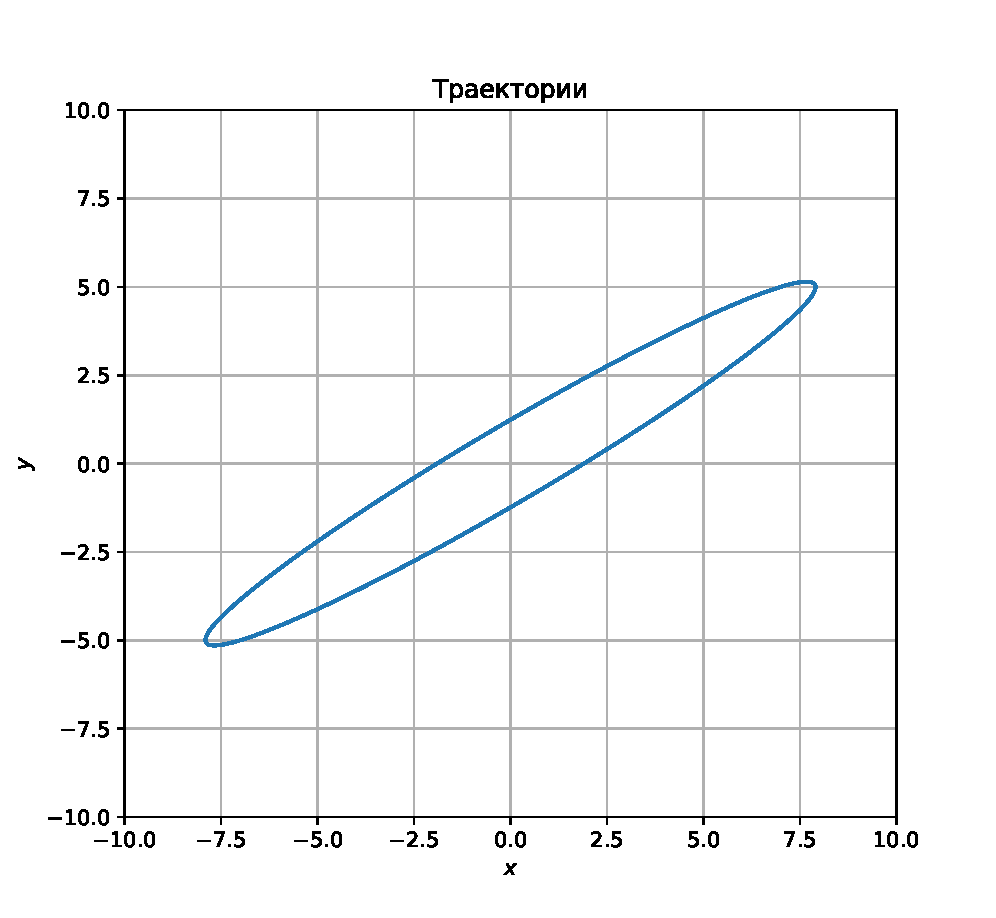
\includegraphics[width=0.5\linewidth]{b0.pdf}
    }
    \caption{Траектория шарика, с нулевым трением}
    \label{b0}
\end{figure}

Если трение присутствует и выполнено условие уравнения (\ref*{uslov}), 
то траектория имеет
вид как на Рис. \ref*{b2less4a}

\begin{figure}[h!!!]
    \noindent\centering{
        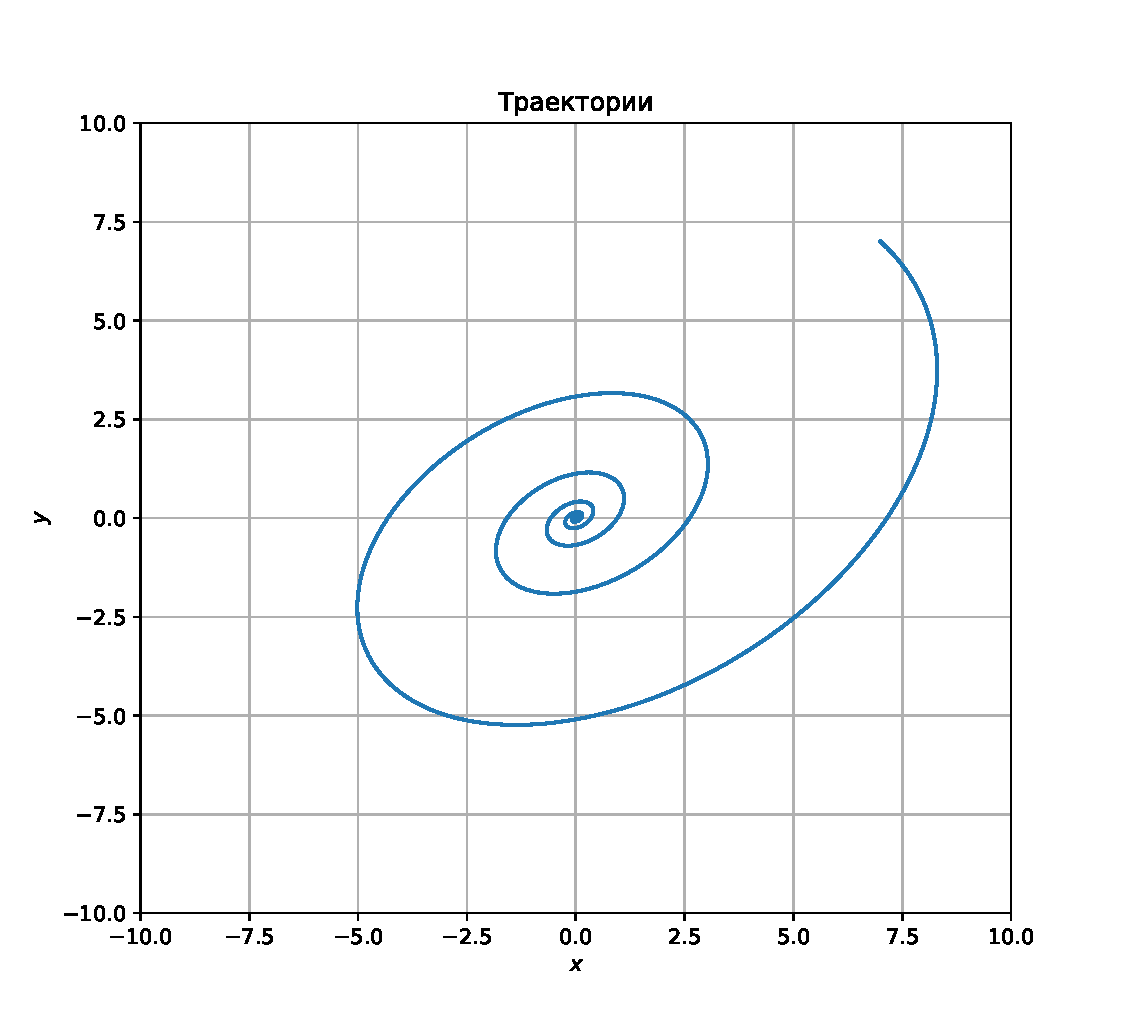
\includegraphics[width=0.5\linewidth]{b2less4a.pdf}
    }
    \caption{Угасающие колебания}
    \label{b2less4a}
\end{figure}
Иначе, при невыполнении условия (\ref*{uslov}), как на Рис. \ref*{b2larg4a} 
\begin{figure}[h!!!]
    \noindent\centering{
        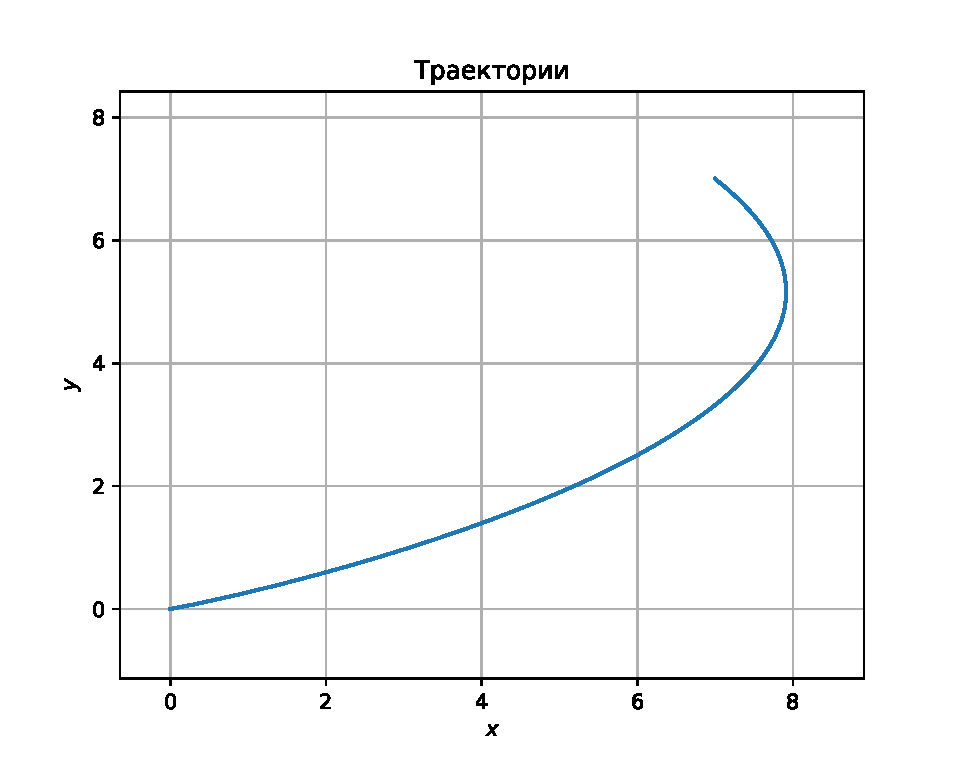
\includegraphics[width=0.5\linewidth]{b2large4a.pdf}
    }
    \caption{Падение без колебаний}
    \label{b2larg4a}
\end{figure}
\subsection{Фазовые портреты}
На Рис. \ref*{faz} представленны характерные фазовые 
портреты при увеличении трения 
и уменьшении жесткости пружины. Происходит плавный переход от спиралей к параболам
\begin{figure}[h!!!]
    \begin{minipage}[h]{0.49\linewidth}
    \center{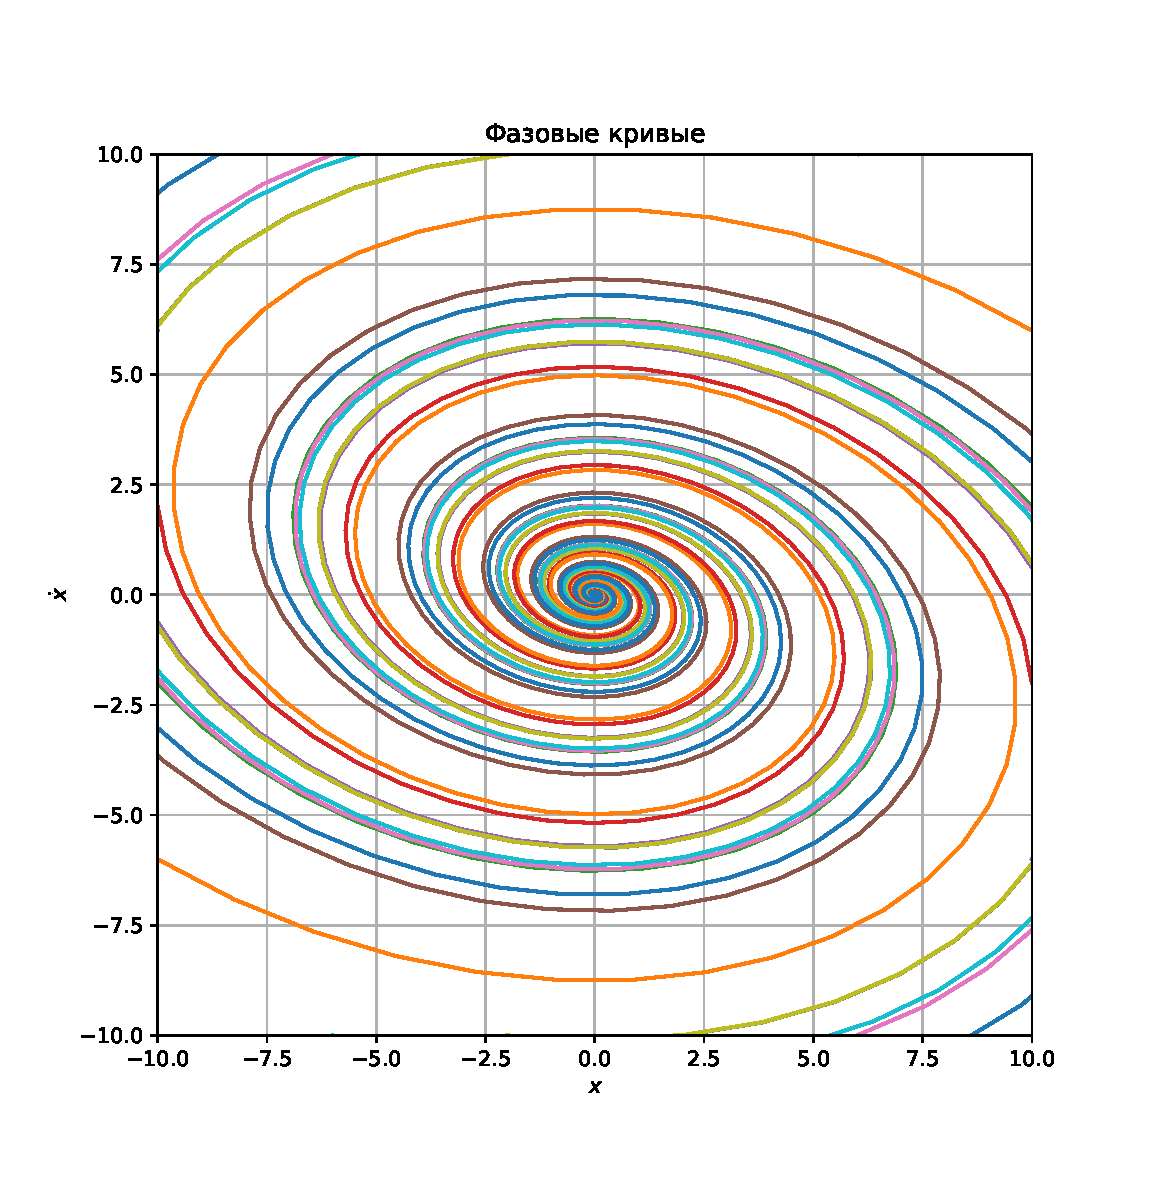
\includegraphics[width=1\linewidth]{faz11.eps} \\ Логарифмические спирали}
    \end{minipage}
    \hfill
    \begin{minipage}[h]{0.49\linewidth}
    \center{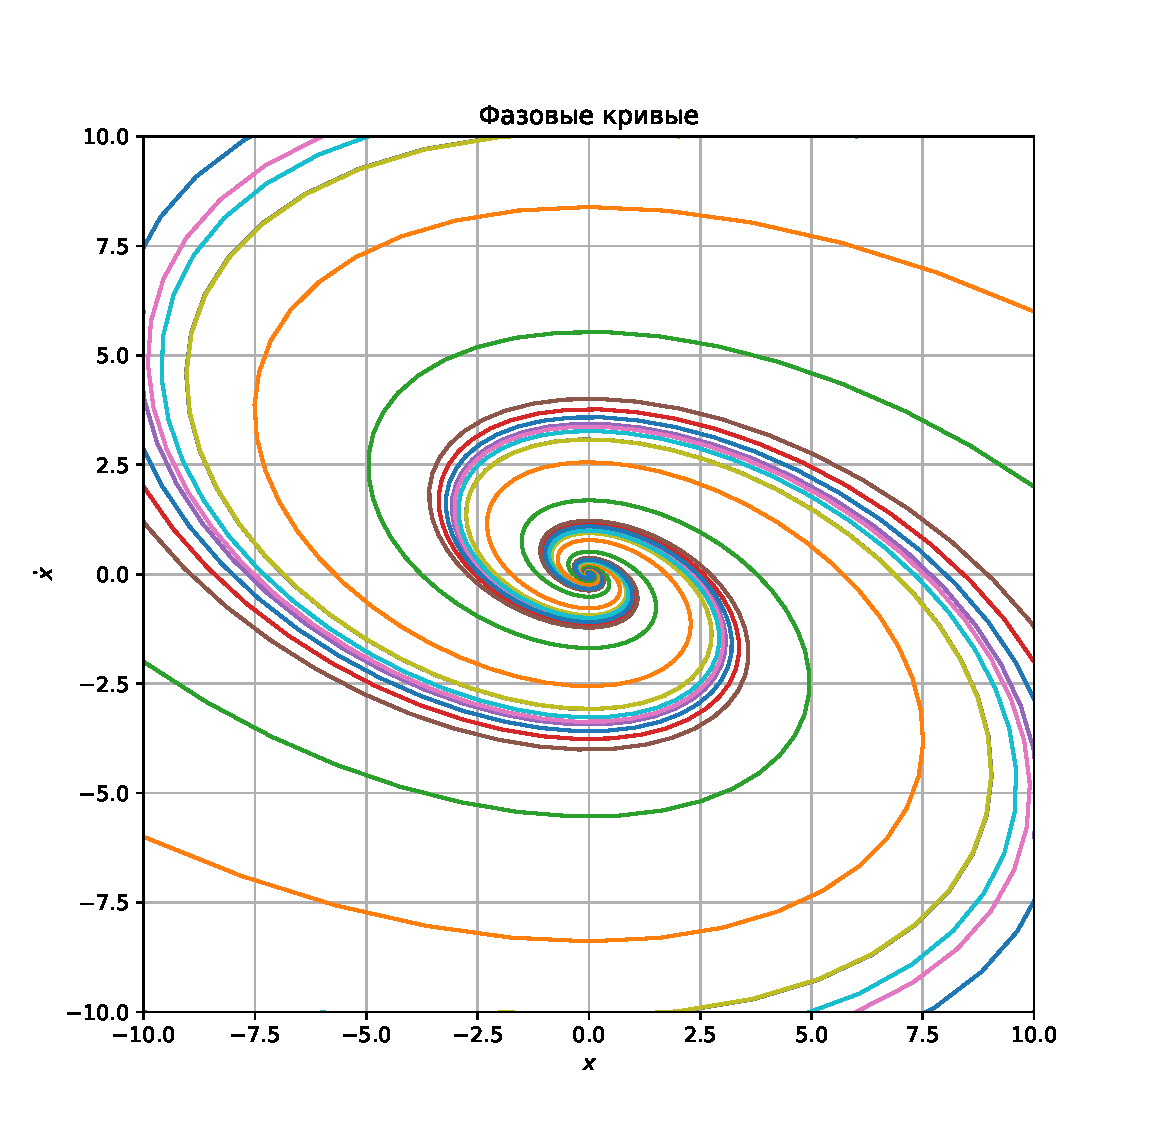
\includegraphics[width=1\linewidth]{faz1.pdf} \\ Логарифмические спирали}
    \end{minipage}
    \hfill
    \begin{minipage}[h]{0.49\linewidth}
    \center{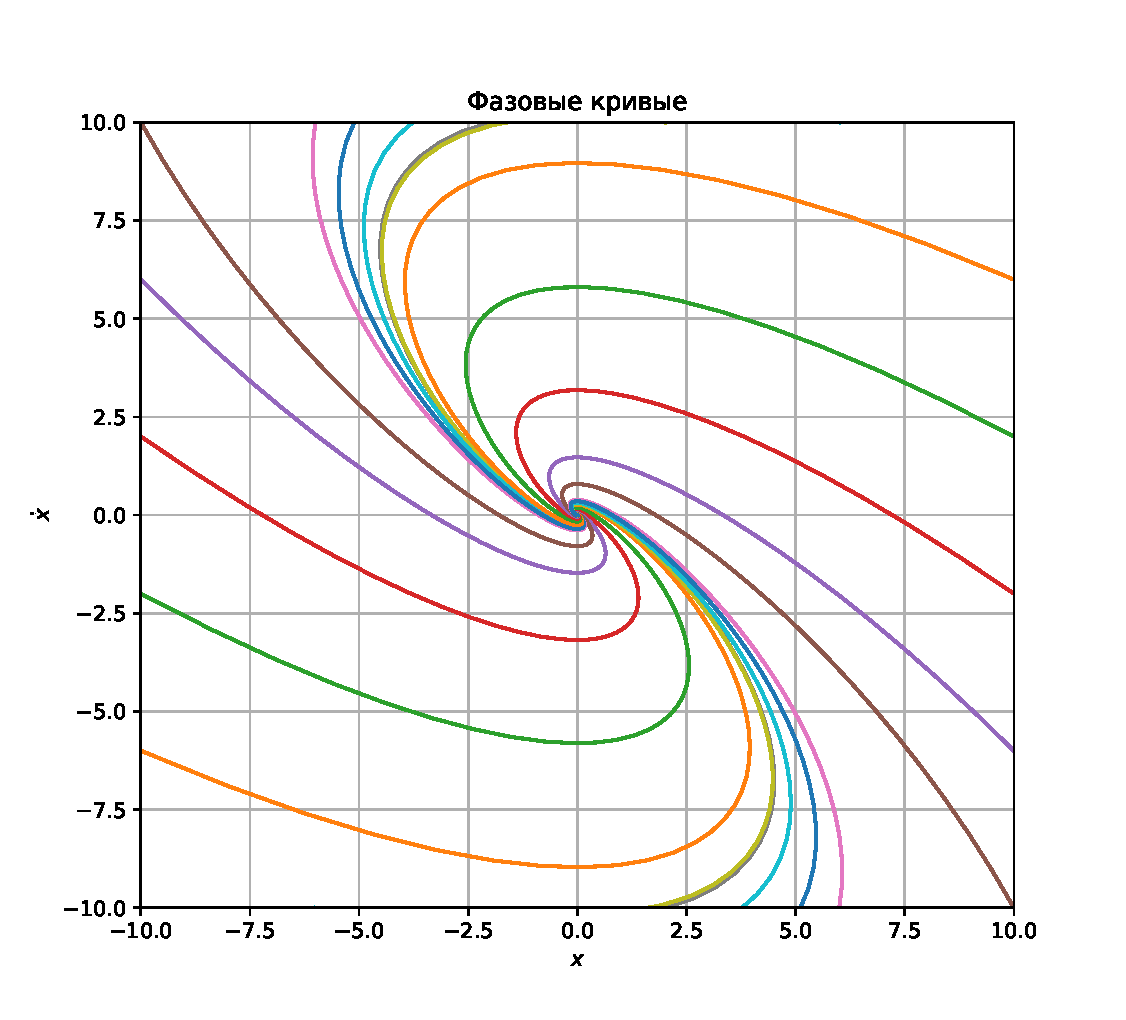
\includegraphics[width=1\linewidth]{faz3.pdf} \\ Параболы}
    \end{minipage}
    \hfill
    \begin{minipage}[h]{0.49\linewidth}
    \center{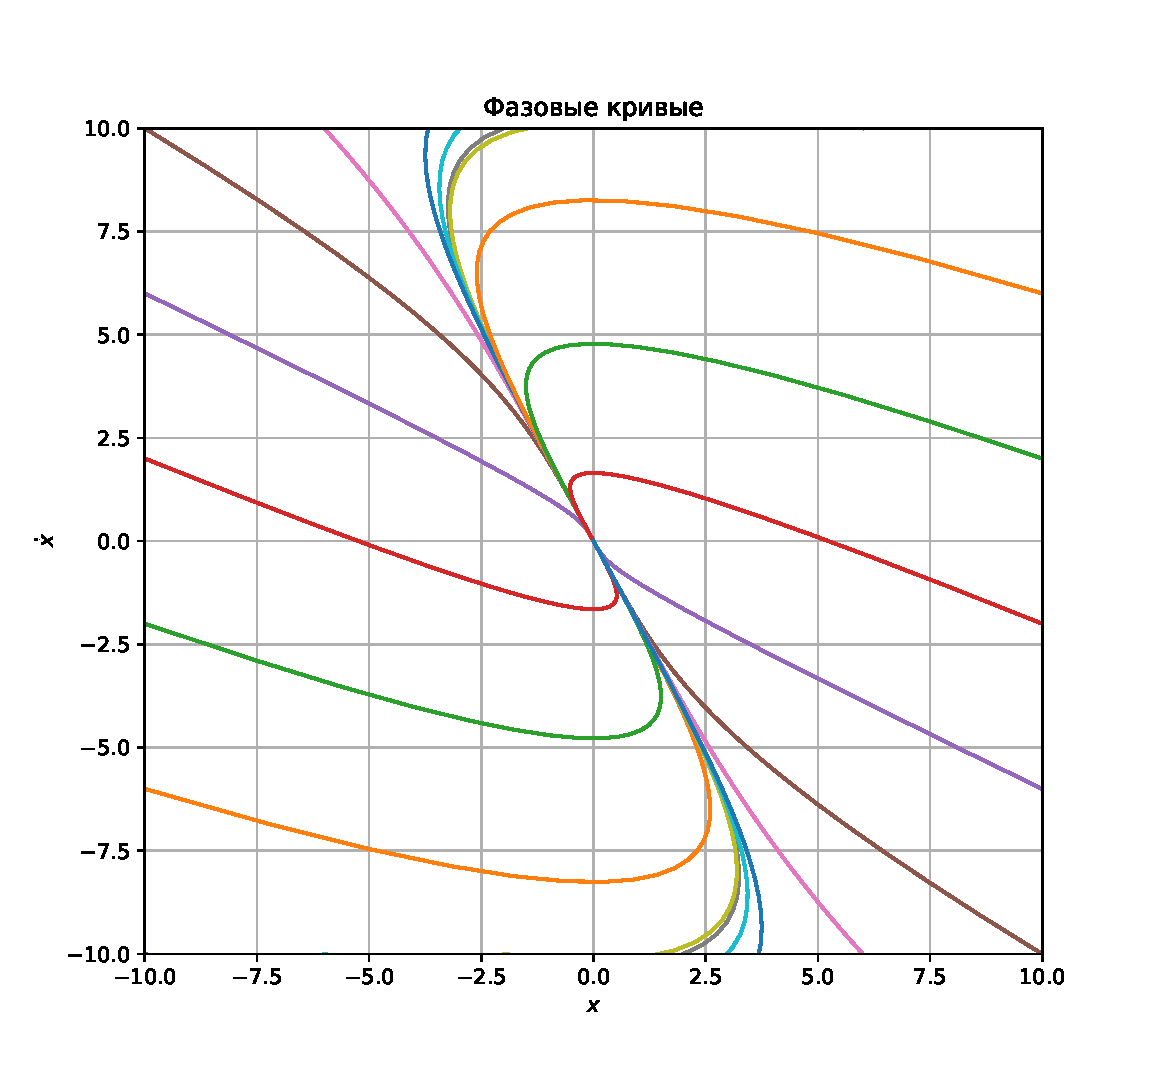
\includegraphics[width=1\linewidth]{faz2.pdf} \\ Параболы}
    \end{minipage}
    \caption{Фазовые партреты при увеличении трения}
    \label{faz}
\end{figure}
\newpage


\newpage
\section{Заключение}
В результате анализа данной нам системы было получено уравнение условия (\ref*{usl}) остуствия 
колебаний в системе. Через параметры системы оно может быть переписано в виде:
\begin{equation}
    b^2 > 4m(k_x + k_y).
\end{equation}
В результате численного моделирования были воспроизведены траектории 
и фазовые портреты, совпадающие с теоретическими полученными.\\
Так же на языке программирования С++ 
были написаны программы для решения системы обыкновенных дифференциальных 
уравнений первого порядка методом Рунге-Кутты четвертого порядка, отрисовки траекторий и фазовых партретов, 
и так же анимации движения шарика и пружин с использованием Виндовс форм.
 \newpage
\begin{thebibliography}{99}
    \addcontentsline{toc}{section}{Список литературы}

    \bibitem{Arn}
    {\bf Арнольд В.И.} Обыкновенные дифференциальные уравнения. – Новое издание, исправл. – М.: МЦНМО, 2012. - 344 c.: 
    ил.ISBN 978-5-94057-907-6 
    \bibitem{cir}
    Автор: Это векторное изображение было создано с помощью Inkscape. 
    - собственная работа, CC BY-SA 3.0, 
    \url{https://commons.wikimedia.org/w/index.php?curid=6947676}
    \bibitem{log}
    Автор: Это векторное изображение было создано с помощью Inkscape. 
    - собственная работа, Общественное достояние, 
    \url{https://commons.wikimedia.org/w/index.php?curid=6990209}
    \bibitem{par}
    Автор: Это векторное изображение было создано с помощью Inkscape. 
    - собственная работа, CC BY-SA 3.0, 
    \url{https://commons.wikimedia.org/w/index.php?curid=6951695}

    \bibitem{all}
    Автор: Maschen - Собственная работа, CC0, 
    \url{https://commons.wikimedia.org/w/index.php?curid=21301479}
    

    

\end{thebibliography}
\end{document}
